\chapter{STM32WB5MM-DK razvojni sustav}

Razvojni sustav temelji se na STM32WB5MMG modulu tvrtke \textit{STMicroelectronics}, koji je dio linije STM32WBx5 razvojnih sustava. Kao i svi mikrokontroleri iz te skupine, modul sadrži 32-bitni Arm Cortex-M4, aplikacijski procesor koji radi na frekvenciji do 64 MHz, te Cortex-M0+, mrežni procesor s frekvencijom rada do 32 MHz. Modul sadrži 1 MB \textit{Flash} memorije i 256 KB SRAM-a. Budući da je modul RF primopredajnik, podržava protokole Bluetooth, Zigbee, Thread i konkurentne bežične standarde. Sustav također ima 0.96-inčni 128x64 zaslon, RGB LED lampice te senzore za temperaturu, dodir, I2C, \textit{Time-of-Flight} senzor i žiroskop. Od ostale periferije najznačajniji je digitalni MEMS mikrofon. STM32 modul je višeprotokolni, bežični uređaj niske potrošnje energije (engl. \textit{ultra-low-power}) primarno namijenjen razvoju aplikacija koje koriste audio, USB ili \textit{Bluetooth Low Energy} (BLE) protokol. 

\begin{figure}[ht]
	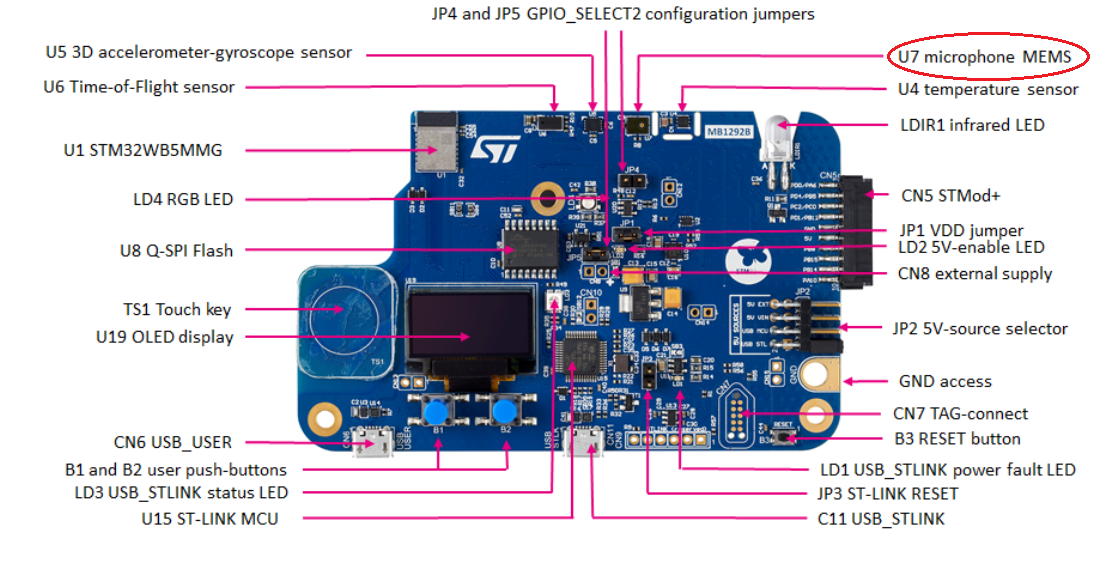
\includegraphics[width=\linewidth]{imgs/discovery_kit}
	\caption{Konfiguracija STM32WB5MM-DK razvojnog sustava}
	\label{fig:discovery-kit}
\end{figure}

\section{BLE protokol}

Bluetooth protokol korišten je za povezivanje razvojnog sustava s matičnim računalom i za prijenos audio signala s mikrokontrolera. BLE je vrsta bežične komunikacije namijenjena komunikaciji kratkog dometa s niskom potrošnjom energije. Razvijen je kako bi se postigao standard vrlo male snage koji radi s baterijom veličine kovanice (engl. \textit{coin-cell batteries}) nekoliko godina.
Klasična Bluetooth tehnologija razvijena je kao bežični standard, što je omogućilo razvoj bežičnih i prenosivih uređaja, no ne podržava dug život baterije zbog brze i nepredvidive komunikacije te složenih postupaka povezivanja. BLE uređaji troše samo dio energije koju troše standardni Bluetooth proizvodi te omogućavaju malenim uređajima s malim baterijama bežično povezivanje s uređajima koji koriste klasični Bluetooth.

BLE radi u istom opsegu od 2,4 GHz kao i standardni Bluetooth, no koristi različite kanale od standardnog Bluetootha. Koristi 40 kanala od 2 MHz za prijenos podataka korištenjem modulacije Gaussova pomaka frekvencije (metoda koja se koristi za glatkije prijelaze između podatkovnih impulsa), zbog čega skokovi frekvencije proizvode manje smetnji u usporedbi sa standardnom Bluetooth komunikacijom.

Arhitektura BLE tehnologije naziva se još i BLE stog zbog slojevite strukture. Stog se sastoji od dvije glavne komponente:
\begin{itemize}
	\item Upravljač (engl. \textit{Controller})
	\item Domaćin (engl. \textit{Host})
\end{itemize}

Upravljač se sastoji od fizičkog sloja i sloja veze. Host uključuje protokol kontrole i prilagodbe logičke veze (L2CAP), upravitelja sigurnosti (SM), protokol atributa (ATT), generički profil atributa (GATT) i generički profil pristupa (GAP). Sučelje između komponenti naziva se sučelje host kontrolera (HCI).


\begin{figure}[ht]
		\centering
		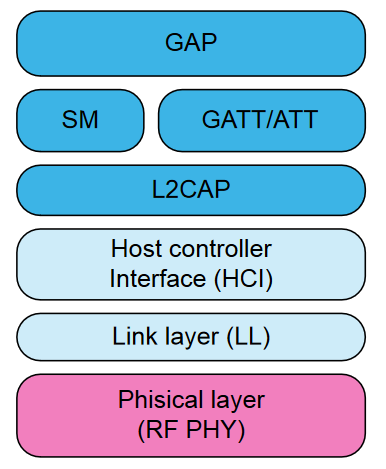
\includegraphics[scale=0.5]{imgs/ble_stack_arch}
		\caption{BLE arhitektura stoga}
		\label{fig:ble-stack-arch}
\end{figure}

\subsection{Upravljač}
\subsubsection{Fizički sloj}
Fizički sloj je radio brzine od 1 Mbps koji prenosi informacije GFSK (\textit{Gaussian Frequency Shift Keying}) frekvencijskom modulacijom. Radi u 2,4 GHz ISM pojasu bez licence na 2400-2483,5 MHz. 
BLE sustav koristi 40 RF kanala (0-39), s razmakom od 2 MHz. Postoje dvije vrste kanala:
\begin{enumerate}
	\item Kanali za oglašavanje koji koriste tri fiksna RF kanala (37, 38 i 39) za
	\begin{enumerate}
		\item Pakete kanala za oglašavanje
		\item Pakete korištene za otkrivanje ili povezivanje
		\item Pakete korištene za odašiljanje ili skeniranje
	\end{enumerate}
	\item Podatkovni fizički kanal, koristi ostalih 37 RF kanala za dvosmjernu komunikaciju između povezanih uređaja.
\end{enumerate}

BLE je tehnologija adaptivnog skakanja frekvencije (AFH) koja može koristiti samo podskup svih dostupnih frekvencija kako bi se izbjegle sve frekvencije koje koriste druge neprilagodljive tehnologije. To omogućuje prelazak s lošeg kanala na poznati dobar kanal korištenjem specifičnog algoritma za skakanje frekvencije, koji određuje sljedeći dobar kanal za korištenje.

\subsubsection{Sloj veze}
Sloj veze određuje kako dva uređaja mogu koristiti radio za međusoban prijenos informacija. Također definira automat s pet stanja:
\begin{itemize}
	\item Stanje pripravnosti (engl. \textit{Standby}): uređaj ne šalje niti prima pakete
	\item Oglašavanje: uređaj šalje oglase putem kanala za oglašavanje
	\item Skeniranje: uređaj traži uređaje oglašivača
	\item Pokretanje (iniciranje): uređaj pokreće vezu s uređajem oglašivača
	\item Veza: uređaj inicijatora u glavnoj je ulozi (engl. \textit{master}) - komunicira s uređajem u podređenoj (engl. \textit{slave}) ulozi i definira vrijeme prijenosa
	\item Uređaj oglašivača je u ulozi podređenog - komunicira s jednim uređajem u glavnoj ulozi 
\end{itemize}

\begin{figure}[ht]
	\centering
	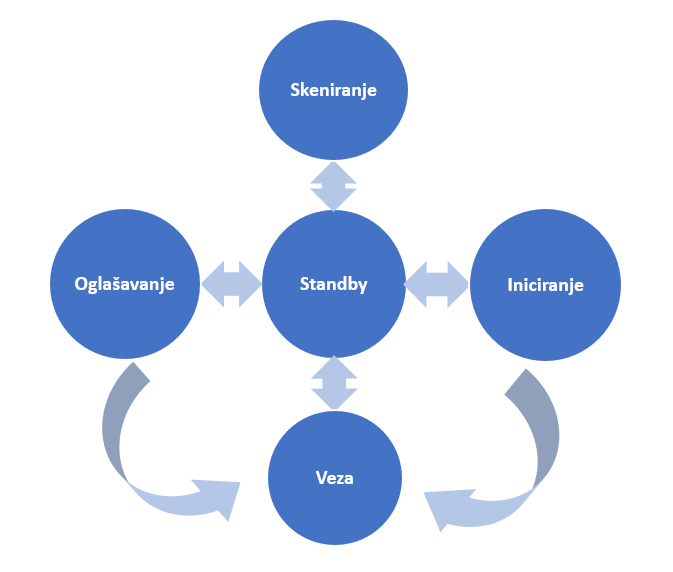
\includegraphics[]{imgs/ll_state_machine}
	\caption{Automat sloja veze}
	\label{fig:ll-state-machine}
\end{figure}

\subsubsection{HCI}
Sloj sučelja glavnog kontrolera (HCI) pruža sredstvo komunikacije između hosta i upravljača  putem softverskog API-ja ili hardverskog sučelja kao što su: SPI, UART ili USB. Dolazi iz standardnih Bluetooth specifikacija, s novim dodatnim naredbama za funkcije specifične uz nisku potrošnju energije.

\subsection{Domaćin}

\subsubsection{L2CAP}
Protokol logičke veze i sloja prilagodbe (L2CAP) podržava multipleksiranje protokola više razine, operacije fragmentacije paketa i ponovnog sastavljanja, te prijenos informacija o kvaliteti usluga.

\subsubsection{ATT}
Protokol atributa (ATT) omogućuje uređaju da prikazuje podatke, koji se nazivaju atributima, drugom uređaju. Uređaj koji prikazuje atribute naziva se poslužiteljem, a uređaj koji ih koristi naziva se klijentom. 
ATT definira skup metoda za otkrivanje, čitanje i pisanje atributa na drugi uređaj. Implementira \textit{peer-to-peer} protokol između poslužitelja i klijenta tipičnom zahtjev-odgovor strukturom. Poslužitelj i klijent imaju sljedeće uloge: 
\begin{itemize}
	\item Poslužitelj
	\begin{itemize}
		\item Sadrži sve atribute (baza atributa)
		\item Prima zahtjeve, šalje odgovore, izvršava naredbe
		\item Obavijesti o promjeni vrijednosti atributa
	\end{itemize}
	\item Klijent
	\begin{itemize}
		\item Komunicira s poslužiteljem
		\item Šalje zahtjeve, čeka na odgovor
		\item Može čitati i mijenjati podatke uz dopuštenje poslužitelja
	\end{itemize}
\end{itemize}

\subsubsection{SM}
BLE sloj veze podržava enkripciju i autentifikaciju korištenjem načina brojača s CBC-MAC algoritmom (kod za provjeru autentičnosti lančanih poruka) i 128-bitnu AES blok šifru (AES-CCM). Kada se enkripcija i autentifikacija koriste u vezi, 4-bajtna provjera integriteta poruke (MIC) dodaje se korisnom učitavanju podatkovnog kanala PDU. Enkripcija se primjenjuje i na polja od PDU i MIC. Kada dva uređaja žele šifrirati komunikacije tijekom veze, upravitelj sigurnosti (SM) koristi postupak uparivanja. Ovaj postupak omogućuje provjeru autentičnosti dvaju uređaja razmjenom informacija o njihovu identitetu kako bi se stvorili sigurnosni ključevi koji se mogu koristiti kao osnova za pouzdani odnos ili (jednu) sigurnu vezu. 

\subsubsection{GATT}
Generički atributni profil (GATT) definira okvir za korištenje ATT protokola, a koristi se za usluge, otkrivanje deskriptora, čitanje, pisanje i obavijesti. U GATT kontekstu, kada su dva uređaja povezana, postoje dvije uloge uređaja:
\begin{itemize}
	\item GATT klijent: uređaj pristupa podacima na udaljenom GATT poslužitelju putem čitanja, pisanja, obavještavanja 
	\item  GATT poslužitelj: uređaj pohranjuje podatke lokalno i pruža metode pristupa podacima udaljenom GATT klijentu
\end{itemize}

Uređaj istovremeno može biti i GATT poslužitelj i GATT klijent.

\subsubsection{GAP}
Bluetooth sustav definira osnovni profil koji implementiraju svi Bluetooth uređaji koji se naziva generički profil pristupa (GAP), koji definira osnovne zahtjeve Bluetooth uređaja. Postoje četiri uloge GAP profila:
\begin{itemize}
	\item Emiter: šalje oglase
	\item Promatrač: prima oglase
	\item Periferija: uvijek u načinu oglašavanja i u \textit{slave} ulozi 
	\item Centar: nikada ne šalje oglase, uvijek u \textit{master} ulozi
\end{itemize}

U kontekstu GAP-a definirana su dva temeljna koncepta:
\begin{itemize}
	\item GAP načini rada (engl. \textit{modes}): konfigurira uređaj da djeluje na određeni način duži vremenski period. Postoje četiri tipa GAP načina rada: emitiranje, otkrivanje, povezivanje i vezanje
	\item GAP procedure: konfigurira uređaj da izvrši jednu radnju u ograničenom vremenskom periodu. Postoje četiri tipa GAP postupaka: promatrač, otkrivanje, povezivanje, postupci povezivanja
\end{itemize}

Istovremeno se mogu koristiti različiti načini otkrivanja i povezivanja.

\section{MEMS mikrofon}

MEMS (\textit{Micro-Electro-Mechanical Systems}) mikrofon je elektroakustični pretvornik koji sadrži MEMS senzor i aplikacijski specifičan integrirani sklop (ASIC). MEMS mikrofoni se uglavnom temelje na elektretskim kapsulama i obično imaju ugrađena pretpojačala i analogno-digitalne pretvornike. MEMS mikrofoni su također poznati kao mikrofonski čipovi ili silikonski mikrofoni.

Svi mikrofoni detektiraju akustične valove pomoću fleksibilne membrane, odnosno dijafragme. Membrana se pomiče pod pritiskom induciranih akustičnih valova. Danas većina MEMS mikrofona na tržištu koristi kapacitivnu tehnologiju za mjerenje zvuka. Kapacitivni MEMS mikrofoni mjere kapacitet između fleksibilne mikromembrane i fiksne stražnje ploče. Promjene tlaka zraka koje stvaraju zvučni valovi uzrokuju pomicanje membrane. Stražnja ploča je perforirana kako bi kroz nju mogao strujati zrak i dizajnirana je da ostane kruta budući da zrak prolazi kroz njezine perforacije. Kako se membrana pomiče, kapacitet se mijenja između pokretne membrane i fiksne stražnje ploče (budući da se udaljenost između njih mijenja), a ta se promjena može analizirati i zabilježiti.

Dizajn digitalnog MEMS mikrofona obično ima dodatni CMOS čip kao analogno-digitalni pretvornik. Ovi čipovi učinkovito preuzimaju pojačane analogne audio signale i pretvaraju ih u digitalne podatke. Također omogućuju lakšu integraciju digitalnih MEMS mikrofona s digitalnim proizvodima.

Najčešći format za digitalno kodiranje unutar MEMS mikrofona je modulacija trajanja impulsa (PDM). PDM omogućuje komunikaciju jednom podatkovnom linijom i satom. Prijemnici PDM signala, kao i sami MEMS mikrofoni, jeftini su i lako dostupni.

\subsection{MEMS tehnologija}
Mikroelektromehanički sustavi ili MEMS je tehnologija koja se definira kao sustav minijaturiziranih mehaničkih i elektromehaničkih elemenata (tj. uređaja i struktura) koji su izrađeni mikrotvorničkim tehnikama. Fizičke dimenzije MEMS uređaja mogu varirati od znatno ispod jednog mikrometra pa sve do nekoliko milimetara. Isto tako, tipovi MEMS uređaja mogu varirati od relativno jednostavnih struktura bez pokretnih elemenata, do iznimno složenih elektromehaničkih sustava s više pokretnih elemenata pod kontrolom integrirane mikroelektronike. Jedan glavni kriterij MEMS-a je da postoje barem neki elementi koji imaju neku vrstu mehaničke funkcionalnosti bez obzira na to mogu li se ti elementi kretati ili ne.

Dok su funkcionalni elementi MEMS-a minijaturizirane strukture, senzori, aktuatori i mikroelektronika, najznačajniji elementi su mikrosenzori i mikroaktuatori. Oni su  kategorizirani kao pretvornici energije iz jednog oblika u drugi - primjerice mikrosenzor, koji obično pretvara izmjereni mehanički signal u električni.

Stvarni potencijal MEMS-a ostvaruje se kada se minijaturizirani senzori, aktuatori i strukture spoje na silicijsku podlogu zajedno s integriranim krugovima, odnosno mikroelektronikom. Dok se elektronika proizvodi pomoću sekvenci procesa integriranog kruga (npr. CMOS, bipolarni ili BICMOS procesi), mikromehaničke komponente proizvode se korištenjem kompatibilnih \textit{micromachining} procesa koji selektivno urezuju dijelove silikonske pločice ili dodaju nove strukturne slojeve kako bi formirali mehaničke i elektromehaničke uređaje. Još je kompleksnije ako se MEMS može spojiti ne samo s mikroelektronikom, već i s drugim tehnologijama kao što su fotonika, nanotehnologija itd. To se ponekad naziva heterogenom integracijom. Dok su složenije razine integracije budući trend MEMS tehnologije, sadašnja je tehnologija skromnija i obično uključuje jedan diskretni mikrosenzor, jedan diskretni mikroaktuator, jedan mikrosenzor integriran s elektronikom, mnoštvo identičnih mikrosenzora integriranih s elektronikom, jedan mikroaktuator integriran s elektronikom ili mnoštvo identičnih mikroaktuatora integriranih s elektronikom. 
 

\subsection{Rad MEMS mikrofona}

MEMS mikrofon sadrži sljedeće komponente:
\begin{itemize}
	\item MEMS pretvornik: sastoji se od membrane, perforirane ploče i ležišta
	\item Isprintana matična ploča (PCB): uključuje ASIC polarizacijsku jedinicu, mikrofonsko pretpojačalo i AD pretvornik
	\item Mehanički poklopac
\end{itemize}

Zvučni valovi ulaze u MEMS mikrofon kroz poklopac i prolaze kroz perforirano kućište i ploču prije nego dođu do membrane. Valovi uzrokuju različiti zvučni tlak na membrani i razliku u tlaku između prednje i stražnje strane membrane. Ova razlika tlaka uzrokuje njeno pomicanje sukladno zvučnim valovima. Međutim, mikrofonski signal se stvara samo ako postoji naboj između vodljive membrane i nepokretne ploče. Ploča i membrana skupa djeluju kao kondenzator koji je potrebno napuniti za ispravan rad. ASIC osigurava ovo punjenje.

Jednom napunjene, ploča i membrana mogu proizvesti napon. Budući da djeluju kao kondenzator, svaka promjena kapaciteta prouzročit će obrnuto proporcionalnu promjenu napona. Kapacitet je funkcija udaljenosti između ploče i membrane, stoga dok membrana oscilira, stvara se izmjenični napon odnosno mikrofonski signal. Ovaj napon treba pojačati da bi bio koristan kao audio signal, stoga odvojeni integrirani krug (poluvodička matrica), uključen u PCB, pojačava signal.

U analognom MEMS mikrofonu, pojačani signal bi se zatim izveo iz MEMS mikrofona i poslao kamo treba ići. Međutim, u digitalnom MEMS mikrofonu postoji dodatni proces u kojem ADC pretvara analogni signal (putem PDM) prije nego što emitira digitalni audio signal.

Kao što se vidi na Slici 2.4., stacionarna ploča je perforirana, što omogućava zraku prolaz do membrane. Na ovom je prikazu ASIC čip pričvršćen na ploču, no to nije slučaj kod svakog MEMS mikrofona. 

Stražnja je komora u ovom primjeru zatvorena, što znači da je MEMS mikrofon tlačni mikrofon - membrana je otvorena samo za zvučne valove s jedne strane, što znači da prima zvuk iz svih smjerova. Stražnja komora također djeluje kao akustični rezonator i tako pomaže pri pravilnom podešavanju mikrofona.

Također je potreban i otvor za ventilaciju kako bi stražnja komora bila pod tlakom okoline.

\begin{figure}[ht]
	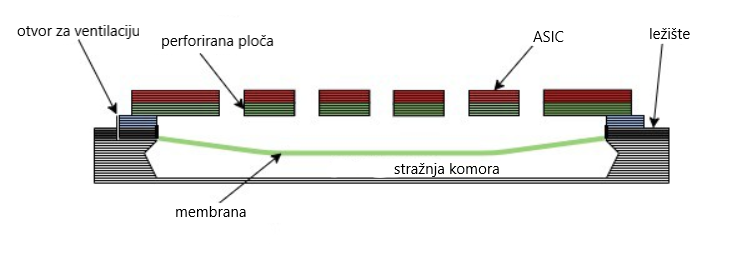
\includegraphics[width=\linewidth]{imgs/mems_mic}
	\caption{Poprečni presjek MEMS mikrofona}
	\label{fig:mems-mic}
\end{figure}